\chapter{设计在费米能级附近的拓扑的平带}

\section{研究背景}

\subsection{拓扑的平带}
电子色散能量局限在狭窄的范围,被推测会呈现一系列有趣的物理现象。这些电子形成密度很高的平带,而在平带
中电子多体效应相对于电子的动能的占据主导地位,此时费米面附近呈现出一种非费米液体,强相互作用的物理效应。物理上
来说,平带可以分为3种,如图\ref{DFBModel}所示。第一种是 the flat atomic bands (FAB),格点上极其局域的轨道,例如格点上
局域的d轨道或者f轨道。由于格点间波函数几乎没有重叠,导致临近的hopping为0,从而产生FAB。这种FAB 在层状和重费米子系统很常见。
第二种是 the flat topological bands (FTB),拥有扩展的波函数,临近格点波函数重叠很大,但是波函数干涉相消导致动能的淬灭。
这种类型的平带在双层扭转石墨烯物理中扮演很重要的角色,它让双层扭转石墨烯同时出现关联的绝缘态和很强耦合的超导,这种超导的相图
非常类似于高温氧化物超导。
第三种是obstructed atomic band (FOAB), 介于前两者之间, 波函数局域在空格点上, 如图\ref{DFBModel}(c)所示。这种类型的平带往往是晶体中的
空位,或者参杂少量其它类型的原子导致的。
由于FTB 具有奇特的性质,让它可以实现很多有趣的量子现象。例如铁磁, Winger晶体, 分数量子霍尔效应,重的费米子, 激子绝缘体态
和激发的量子反常和自旋霍尔效应。尤其最近这种拓扑的平带可以增强双层扭转石墨烯的超流体的比重和可能导致高温超导体。
理想的FTB在晶体中在费米面附近还没有发现。目前实验唯一发现的FTB是在双层扭转石墨烯种,展现一系列有趣的物理现象。然后,由于双层扭转石墨烯
的原包非常大,导致平带电子在 moire样品中的密度非常低,阻碍了人们研究这种与高密度有关的物理现象。
同时目前为止,大量的理论研究者仅仅关心哪个晶格可能会出拓扑的平带,例如Lieb 晶格, Kagome 晶格 和 star 晶格等等。然而,怎么在费米面发现
和构造一个拓扑的平带在那些晶格中,这仍然是需要研究的课题。因此,迫切需要提出一个一般的规则,去寻找在费米面附近的平带。从而加速实验上去发现FTB,
研究FTB相关的物理和利用FTB的性质。

\begin{figure}[htb]
    \centering
    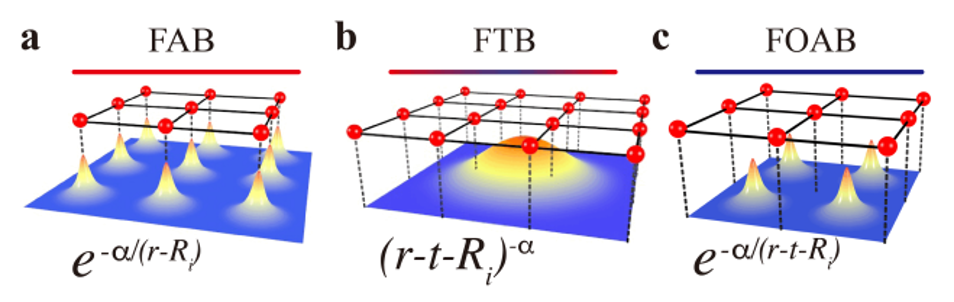
\includegraphics[width=0.9\textwidth]{DFBModel.png}
    \caption{图示3种类型的平带。(a) FAB: 波函数局域在原子格点上。(b) FTB: 波函数局域在特定的晶胞平台内。 (c) FOAB: 波函数局域在空格点上。
    摘自文献。}
    \label{DFBModel}
    \note{}
\end{figure}

\subsection{共价有机框架材料}
共价有机框架材料,是一类具有可设计和可预测结构的结晶多孔有机聚合物,可以通过共价键的有机单元整合构建而成。由于
其周期性骨架、超低密度、高表面积、良好的拓扑结构和多样的功能,共价有机框架材料在化学和材料科学中引起了相当大的关注。
另一方面,二维共价有机框架晶体可以用拓扑方法将结构块的单体组装在刚性骨架中自下而上设计,
因此二维晶体的奇异电子性质可以由单体的前线轨道确定。 在本章中,我们首先揭示了晶体拓扑的平带与晶体单体的前线轨道之间的联系,
并提出了一般的搜索平带规则。此外,具有铁磁共价有机框架材料可以在参杂一定的空穴或者电子浓度时实现,而共价有机框架材料往往是非磁的。
同时考虑floquet的圆偏振光照射,我们可以实现有趣的enantiomorphic anomalous hall effect (EAHE)。这些发现为设计FTB在费米面附近
提供一种新的思路,提供一个新的策略去研究共价有机框架材料自旋电子学。




\section{FTB的紧束缚模型}

\subsection{Kagome 平带}
我们首先介绍Kagome平带。